% --- Packages: core and language (pdfLaTeX)
\usepackage[utf8]{inputenc}
\usepackage[T5]{fontenc}
\usepackage{lmodern}
\usepackage[vietnamese,english]{babel}

% --- Packages: math and symbols
\usepackage{amsmath}
\usepackage{amsthm}
\usepackage{amssymb}
\usepackage[makeroom]{cancel}

% --- Packages: layout and spacing
\usepackage{a4wide}
\usepackage{geometry}
\usepackage{setspace}
\usepackage{changepage}
\usepackage[protrusion=false, nopatch=footnote]{microtype}

% --- Packages: graphics and color
\usepackage{graphicx}
\usepackage{xcolor}
\usepackage{colortbl}
\usepackage{tikz}
\usetikzlibrary{arrows,backgrounds,decorations.pathmorphing}
\usepackage{eso-pic}

% --- Packages: floats, captions, and subfigures
\usepackage{float}
\usepackage{caption}
\usepackage{subcaption}

% --- Packages: tables and columns
\usepackage{array}
\usepackage{tabularx}
\usepackage{multirow}
\usepackage{multicol}
\usepackage{makecell}
\usepackage{rotating}
\usepackage{booktabs}
\usepackage{hhline}

% --- Packages: text and lists
\usepackage{enumitem}
\usepackage{soul}
\usepackage{verbatim}
\usepackage[normalem]{ulem}

% --- Packages: code and algorithms
\usepackage{listings}
\usepackage{matlab-prettifier}
\usepackage[lined,boxed,commentsnumbered]{algorithm2e}
\usepackage[many]{tcolorbox}

% --- Packages: headers, references, and utilities
\usepackage{fancyhdr}
\usepackage{lastpage}
\usepackage[first=0,last=9]{lcg}
\usepackage{latexsym}

% --- Hyperref (keep near the end)
\usepackage{hyperref}
\hypersetup{
    urlcolor=blue,
    linkcolor=black,
    citecolor=black,
    colorlinks=true
}

% --- Background image helper
\newcommand\BackgroundPic{
    \put(0,0){
        \parbox[b][\paperheight]{\paperwidth}{
            \vfill
            \centering
            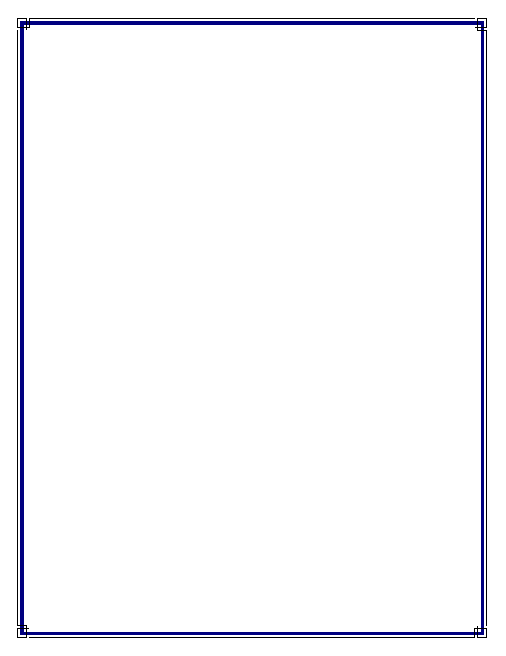
\includegraphics[
                width=\paperwidth,
                height=\paperheight,
                keepaspectratio
            ]{image/assets/background.png}
            \vfill
        }
    }
}

% --- Global numbering and spacing
\setlength{\parindent}{0pt}
\numberwithin{equation}{section}
\numberwithin{figure}{section}

% --- Listings: styles
\lstdefinestyle{defaultCode}{
    language=C,
    basicstyle=\ttfamily\small,
    numbers=left,
    numberstyle=\tiny\color{gray},
    stepnumber=1,
    numbersep=8pt,
    keywordstyle=\color{blue}\bfseries,
    stringstyle=\color{red},
    showstringspaces=false,
    commentstyle=\color{teal},
    breaklines=true,
    frame=single,
    tabsize=4,
    captionpos=b
}

\definecolor{projectbg}{RGB}{245,248,255}
\lstdefinestyle{projecttree}{
    basicstyle=\ttfamily\small,
    columns=fullflexible,
    showstringspaces=false,
    keepspaces=true,
    frame=single,
    backgroundcolor=\color{projectbg},
    morecomment=[l]{\#},
    commentstyle=\color{gray}
}

\colorlet{codebg}{yellow!5!white}
\definecolor{codeframe}{RGB}{0,0,0}
\definecolor{codekw}{RGB}{38,92,190}
\definecolor{codestring}{RGB}{196,74,116}
\definecolor{codecomment}{RGB}{106,153,85}
\definecolor{codenumber}{RGB}{150,150,150}

\lstdefinestyle{espCode}{
    language=C,
    basicstyle=\ttfamily\small,
    numbers=left,
    numberstyle=\tiny\color{codenumber},
    stepnumber=1,
    numbersep=8pt,
    keywordstyle=\color{codekw}\bfseries,
    stringstyle=\color{codestring},
    commentstyle=\color{codecomment}\itshape,
    backgroundcolor=\color{codebg},
    frame=single,
    rulecolor=\color{codeframe},
    breaklines=true,
    tabsize=4,
    captionpos=b,
    keepspaces=true,
    showstringspaces=false
}

% --- Listings: active style
\lstset{style=espCode}